\chapter{Analyse et Spécification des Besoins}

\section{Introduction}
La phase de spécification des besoins constitue le fondement de tout projet
informatique réussi. Elle consiste à définir avec rigueur \textit{ce que le système doit
accomplir}, avant d'aborder \textit{comment il va le faire}. Dans ce chapitre, nous
identifierons les acteurs du système, listerons les exigences fonctionnelles et
non-fonctionnelles, puis modéliserons ces interactions à l'aide du langage \textbf{UML}
(Unified Modeling Language)~\cite{roques2006}.

\section{Identification des Acteurs}
Un acteur représente une entité externe qui interagit directement avec le système.
Notre analyse du terrain a permis d'identifier trois rôles distincts, chacun avec un
périmètre d'action bien délimité :
\begin{itemize}
    \item \textbf{L'Employé (Reporter/Demandeur) :} Agent de la Branche Carburants
    utilisant les applications informatiques. Il crée les tickets d'incidents et consulte
    uniquement l'état d'avancement de \textit{ses propres} requêtes.
    \item \textbf{Le Technicien (Support) :} Membre de l'équipe du Groupe Informatique.
    Il consulte la file d'attente des tickets non assignés, s'assigne volontairement des
    tickets, met à jour leur statut et rédige des rapports de diagnostic.
    \item \textbf{L'Administrateur :} Superviseur du système, disposant d'un
    « pouvoir absolu ». Il peut forcer l'assignation ou la réassignation des tickets,
    gérer l'ensemble des comptes utilisateurs et consulter les tableaux de bord
    statistiques globaux (KPIs).
\end{itemize}

\section{Spécification des Besoins}

\subsection{Besoins Fonctionnels}
Les besoins fonctionnels décrivent les services que le logiciel doit rendre. Notre
système doit permettre :
\begin{enumerate}
    \item \textbf{Authentification sécurisée} basée sur le rôle (Reporter, Technicien,
    Administrateur).
    \item \textbf{Création d'un ticket} par le Demandeur : formulaire structuré avec
    titre, description détaillée, catégorie d'application, niveau de priorité (Critique,
    Majeur, Mineur) et pièces jointes (captures d'écran).
    \item \textbf{Consultation de la file d'attente} par le Technicien : liste des
    tickets ouverts et non assignés, filtrables et triables.
    \item \textbf{Assignation dynamique} : prise en charge volontaire par le technicien
    (bouton « S'assigner ») ou affectation forcée par l'Administrateur.
    \item \textbf{Gestion du cycle de vie} du ticket : transitions de statut avec
    commentaires obligatoires lors de la clôture (\textit{Résolu} ou \textit{Échec}).
    \item \textbf{Logique de retour en file} : si un technicien remet un ticket à
    l'état « Ouvert », le système désassigne automatiquement le technicien et replace
    le ticket dans la file globale.
    \item \textbf{Tableau de bord dynamique} : affichage en temps réel de KPIs
    générés par des requêtes SQL agrégées (nombre de tickets par statut, par
    priorité, par technicien).
    \item \textbf{Journal d'audit complet} : chaque action (création, changement de
    statut, commentaire) est horodatée et tracée dans la table \texttt{incident\_logs}.
\end{enumerate}

\subsection{Besoins Non-Fonctionnels}
Ces besoins définissent les contraintes de qualité, d'environnement et de service. Ils
s'inscrivent dans la continuité des analyses sur la performance des fonctions support dans
les grandes organisations~\cite{meghari2014,autissier2008} : un outil peut être fonctionnellement
correct et pourtant inadapté s'il n'est pas utilisable, maintenable ou aligné sur
l'infrastructure d'entreprise.

\subsubsection{Infrastructure et compatibilité}
La plateforme doit s'exécuter sur \textbf{Windows Server 2019} avec \textbf{IIS} et
\textbf{FastCGI} pour PHP, et utiliser \textbf{Microsoft SQL Server} (édition Express acceptable
pour un périmètre pilote), conformément aux standards Naftal. Les navigateurs cibles sont les
navigateurs courants du parc (Edge, Chrome) en mode intranet.

\subsubsection{Ergonomie et expérience utilisateur}
L'interface doit limiter la charge cognitive : libellés en français, hiérarchie visuelle claire
(Bootstrap~5), tableaux triables (DataTables), formulaires validés côté serveur avec messages
d'erreur explicites. Le \textbf{Responsive Web Design} permet l'usage sur poste fixe ou portable
lors des astreintes ou déplacements internes.

\subsubsection{Sécurité}
Outre sessions PHP et \texttt{requireRole()}, les mots de passe sont stockés exclusivement sous
forme de \textbf{hash} (\texttt{password\_hash} / \texttt{password\_verify}). Les accès données
passent par \textbf{PDO} et des paramètres liés. Les fichiers uploadés ne doivent pas être
exécutables comme scripts ; le répertoire dédié fait l'objet de droits restreints côté serveur.

\subsubsection{Disponibilité et continuité de service}
L'application vise une disponibilité \textbf{24h/24} sur le réseau intranet de la Branche, sous
réserve de la disponibilité du serveur et de la base (plan de sauvegarde et restauration hors
périmètre fonctionnel mais documenté en déploiement).

\subsubsection{Performance et scalabilité indicielle}
Pour un volume «\,branche\,» de tickets, les requêtes d'agrégation pour les KPIs doivent rester
sous des seuils acceptables sur SQL Server Express ; des index sur les colonnes de filtrage
(\texttt{status}, \texttt{assigned\_to}, dates) sont prévus en conception. Une montée en charge
ultérieure pourrait passer par une édition Standard / cluster, hors objet du présent mémoire.

\subsubsection{Maintenabilité et évolutivité}
Le découpage en scripts PHP par responsabilité (\texttt{actions/}, pages vues) facilite les
corrections. L'ajout de champs métier (ex.\ sous-catégorie) doit pouvoir se faire sans refonte
complète grâce au schéma relationnel documenté.

\subsubsection{Traçabilité et conformité procédurale}
Chaque action significative génère une ligne de journal : exigence non fonctionnelle \emph{critique}
pour les audits internes et la confiance entre services — elle conditionne la valeur probante du
système.

\subsubsection{Récapitulatif des contraintes non fonctionnelles}
\begin{table}[H]
\centering
\small
\begin{tabular}{@{}p{4cm}p{10cm}@{}}
\toprule
\textbf{Attribut de qualité} & \textbf{Attendu mesurable ou vérifiable} \\
\midrule
Infrastructure & Windows Server 2019, IIS, PHP~8, SQL Server, PDO\_SQLSRV. \\
Utilisabilité & Parcours création ticket $\leq$ quelques minutes pour un utilisateur guidé. \\
Sécurité & Pas de mot de passe en clair en base ; pas d'injection SQL sur scénarios de test manuels. \\
Disponibilité & Service joignable sur VLAN intranet selon fenêtre d'exploitation du serveur. \\
Performance & Listes et KPIs utilisables sans délai perceptible sur jeu de test représentatif. \\
Auditabilité & Historique complet reconstituable pour un ticket donné via \texttt{incident\_logs}. \\
\bottomrule
\end{tabular}
\caption{Synthèse des attributs de qualité non fonctionnels}
\label{tab:nfr}
\end{table}

\section{Modélisation UML : Diagramme des Cas d'Utilisation}
Le diagramme de cas d'utilisation (Use Case) est l'outil UML de référence pour
formaliser les interactions entre les acteurs et le système~\cite{roques2006}.

\begin{figure}[H]
    \centering
     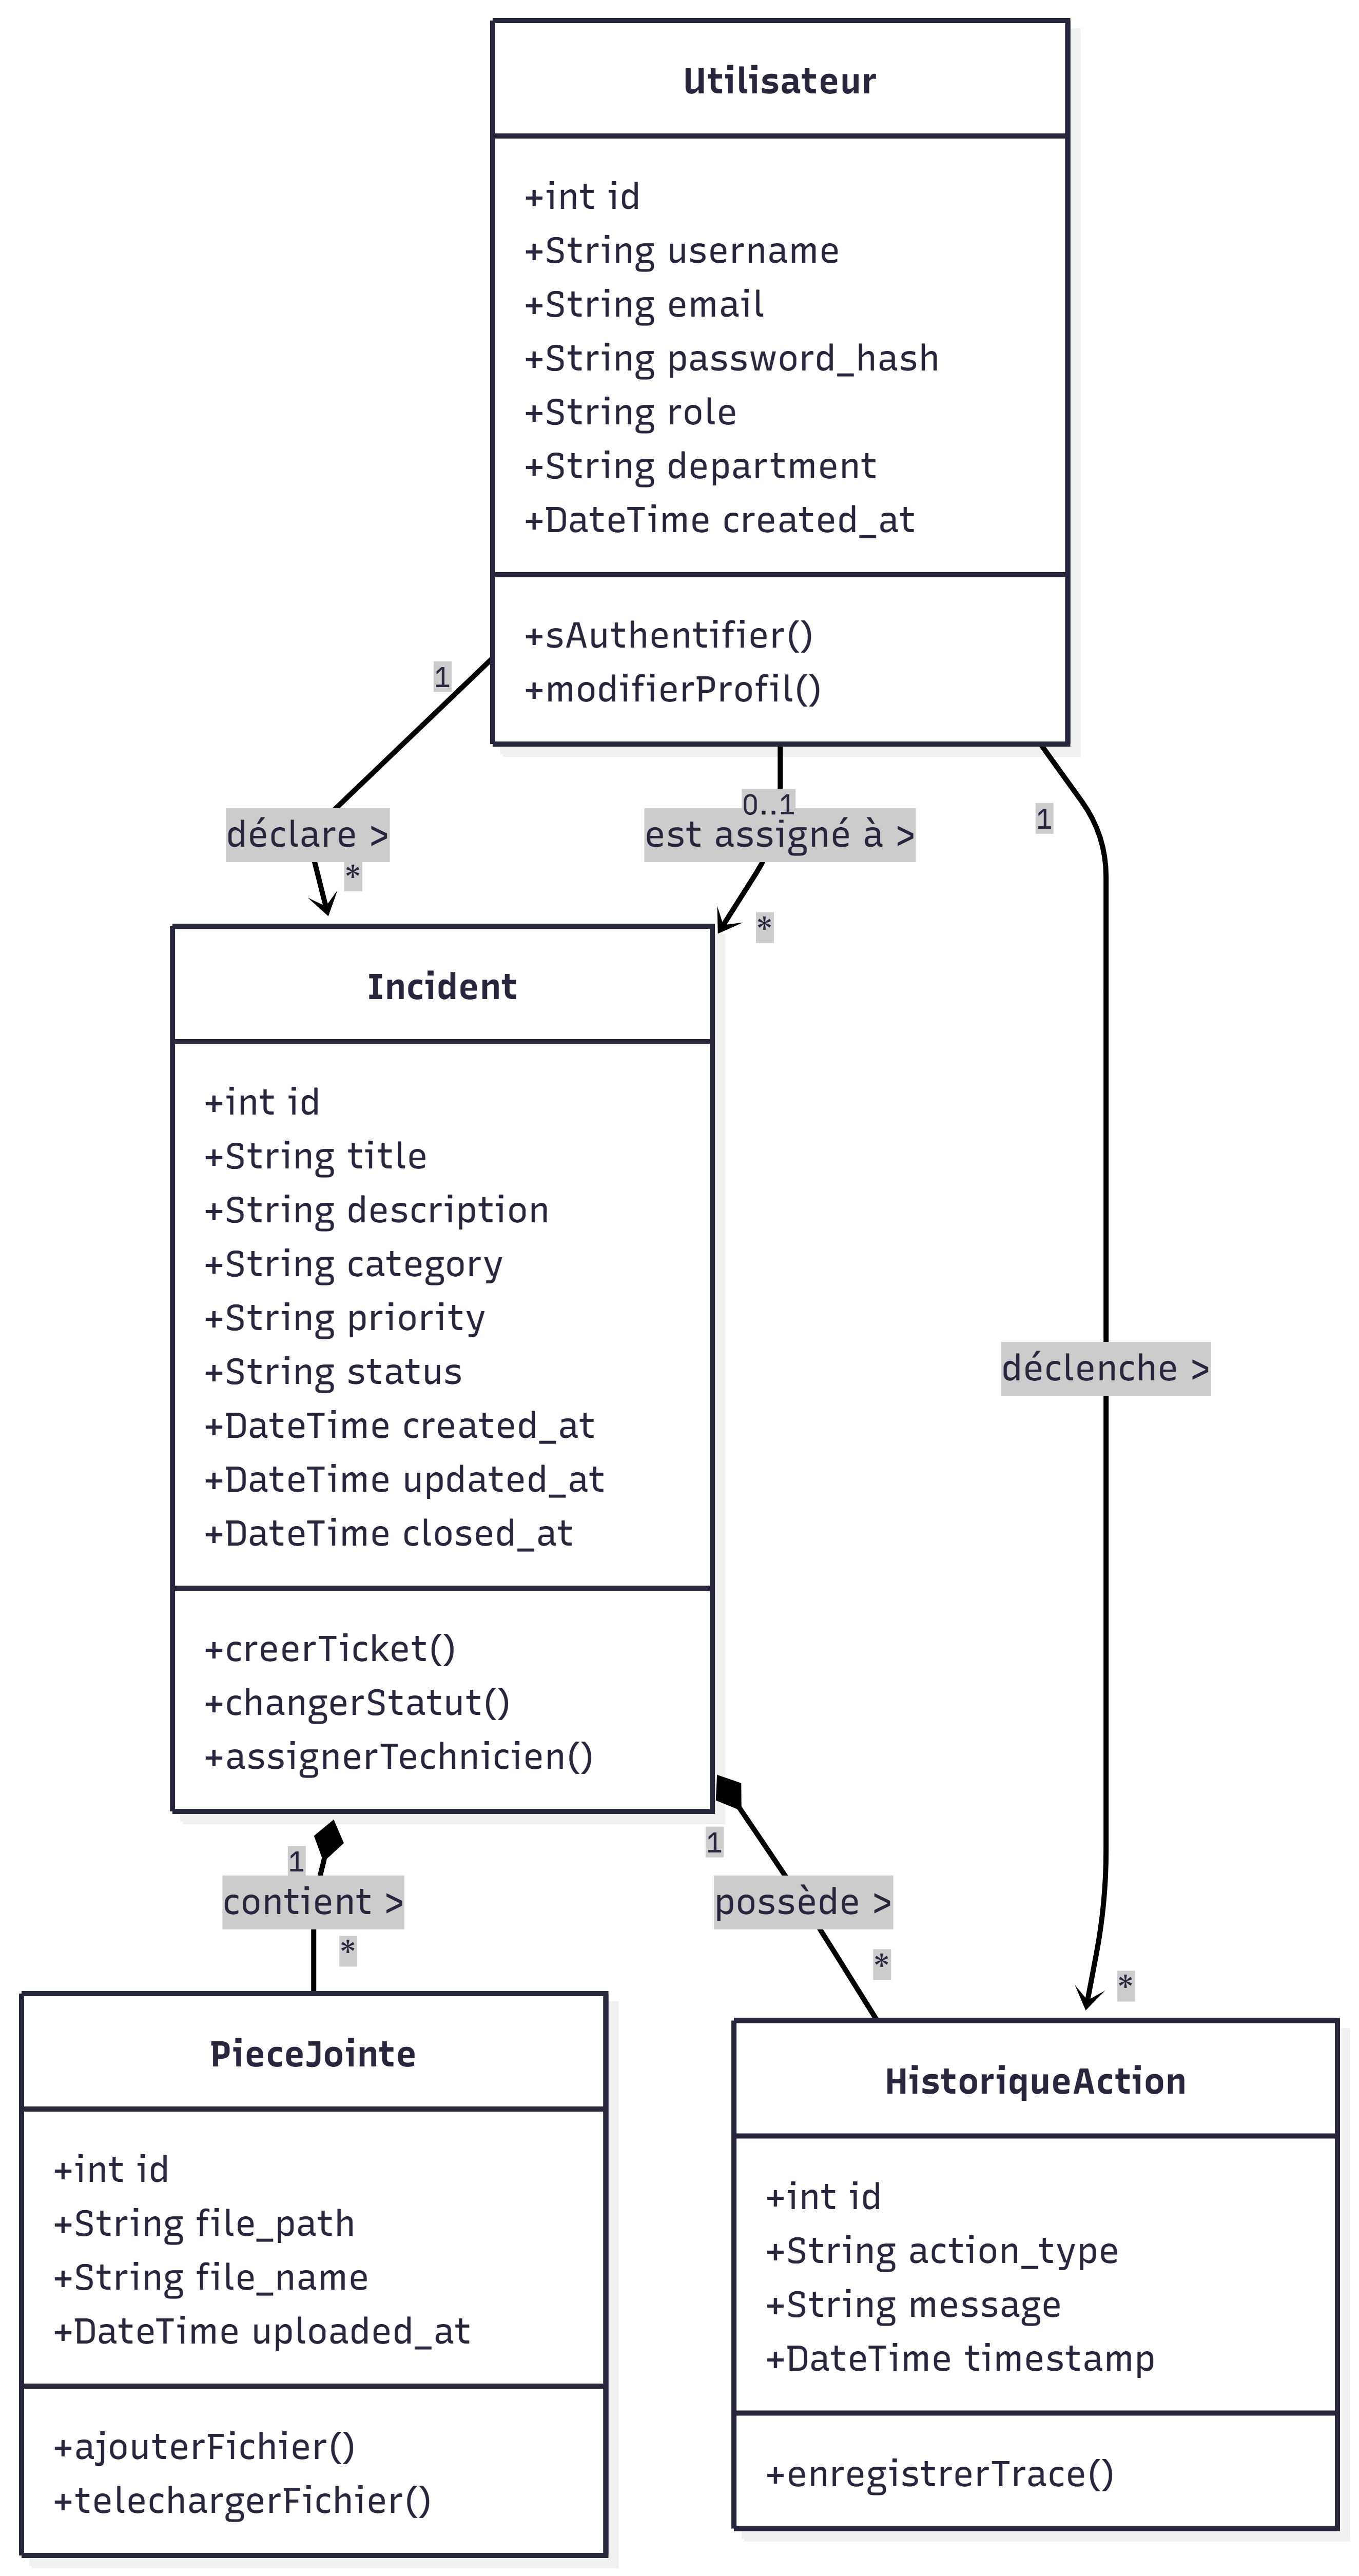
\includegraphics[width=0.5\textwidth]{figures/diagramme_use_case.png}
    \caption{Diagramme des Cas d'Utilisation de la plateforme GIA}
    \label{fig:usecase}
\end{figure}

Le diagramme illustre la séparation stricte des \textbf{privilèges} selon les rôles : le
Demandeur ne modifie pas les tickets des autres ; le Technicien agit sur la file et sur les
tickets qui lui sont associés ; l'Administrateur dispose de capacités d'assignation et de
supervision globale (tableaux de bord, gestion des comptes). Cette structuration réduit le
risque d'actions non autorisées et simplifie la politique de sécurité (contrôle d'accès par
rôle, décrit en conception).

\section{Description textuelle des cas d'utilisation principaux}
Pour lever toute ambiguïté sur le diagramme, les scénarios suivants résument le comportement
attendu du système (formulation \textit{happy path} ; les exceptions — session expirée, droits
insuffisants — sont traitées côté serveur) :

\subsection{Authentification}
\textbf{Acteur :} tout utilisateur disposant d'un compte. \textbf{Flux :} saisie des identifiants ;
vérification du mot de passe haché ; création de session ; redirection vers l'écran adapté au
rôle (Employé, Technicien ou Administrateur).

\subsection{Créer un ticket d'incident}
\textbf{Acteur :} Employé. \textbf{Flux :} ouverture du formulaire ; saisie du titre, de la
description, de la catégorie et de la priorité ; éventuelle pièce jointe ; enregistrement avec
statut initial \texttt{Ouvert} ; écriture d'une ligne \texttt{Creation} dans le journal d'audit.

\subsection{Prendre en charge un ticket}
\textbf{Acteur :} Technicien. \textbf{Flux :} consultation de la file ; sélection d'un ticket non
assigné ; action « S'assigner » ; passage au statut \texttt{Assigné} ; journalisation de
l'assignation.

\subsection{Faire évoluer le statut et clôturer}
\textbf{Acteur :} Technicien (ou Administrateur selon les mêmes règles métier). \textbf{Flux :}
choix du nouveau statut (\texttt{Diagnostic}, \texttt{Résolu}, \texttt{Clos},
\texttt{Échec/Bloqué}, ou retour \texttt{Ouvert}) ; si clôture ou échec, saisie d'un commentaire
obligatoire ; mise à jour des horodatages ; journalisation.

\subsection{Superviser et réassigner}
\textbf{Acteur :} Administrateur. \textbf{Flux :} consultation des indicateurs agrégés ;
réassignation d'un ticket à un autre technicien si nécessaire ; administration des comptes
utilisateurs.

\section{Scénarios dynamiques (logique de séquence)}
Sans reproduire ici l'intégralité des diagrammes de séquence UML, nous détaillons les
\textbf{enchaînements} entre \textit{Acteur}, \textit{Interface}, \textit{Contrôleur PHP} et
\textit{Base de données}, conformément au langage UML~\cite{roques2006}.

\subsection{Séquence «\,Connexion\,»}
\begin{enumerate}
    \item L'utilisateur saisit identifiant et mot de passe ; le navigateur envoie une requête
    \texttt{POST} vers le script d'authentification.
    \item PHP récupère l'enregistrement utilisateur ; compare le hash ; en cas de succès crée
    la session (\texttt{\$\_SESSION}) avec identifiant et rôle.
    \item Redirection vers le tableau de bord ou la page d'accueil du rôle ; en cas d'échec,
    message générique (sans révéler si l'identifiant existe).
\end{enumerate}

\subsection{Séquence «\,Soumettre un ticket\,»}
\begin{enumerate}
    \item L'Employé remplit le formulaire et valide ; éventuel \texttt{multipart/form-data} pour
    les pièces jointes.
    \item PHP contrôle le rôle \emph{Reporter}, valide les champs obligatoires, enregistre la ligne
    \texttt{incidents} avec statut \texttt{Ouvert}.
    \item Insertion d'une entrée \texttt{Creation} dans \texttt{incident\_logs} ; enregistrement
    du fichier sur disque si présent.
    \item Retour utilisateur : confirmation et numéro de ticket ou message d'erreur explicite.
\end{enumerate}

\subsection{Séquence «\,Changer le statut\,»}
\begin{enumerate}
    \item Le Technicien soumet le formulaire de mise à jour ; \texttt{update\_ticket.php} vérifie
    session, rôle et droit sur le ticket (assigné ou administrateur).
    \item Transaction logique : mise à jour \texttt{incidents} (statut, dates, \texttt{assigned\_to}
    si retour \texttt{Ouvert}) ; insertion journal.
    \item Rechargement de la vue ticket : timeline reconstruite à partir de \texttt{incident\_logs}.
\end{enumerate}

\subsection{Vue d'ensemble couche à couche}
Le navigateur n'accède jamais directement au SGBD : toute requête SQL transite par PHP, ce qui
matérialise le principe de \textbf{délégation} de la couche présentation vers la couche métier,
elle-même seule habilitée à parler au stockage — architecture développée au chapitre suivant.

\section{Règles de gestion et invariants métier}
Le tableau~\ref{tab:regles} formalise des invariants qui doivent rester vérifiés après toute
évolution du code (tests de recette).

\begin{table}[H]
\centering
\small
\begin{tabular}{@{}p{1cm}p{13cm}@{}}
\toprule
\textbf{ID} & \textbf{Règle} \\
\midrule
R1 & Un ticket nouvellement créé est \texttt{Ouvert} et \texttt{assigned\_to} est nul. \\
R2 & Seul un Technicien ou un Admin peut passer un ticket à \texttt{Assigné} ou au-delà. \\
R3 & Un Employé ne consulte que les tickets dont il est le créateur (\texttt{user\_id}). \\
R4 & Tout passage à \texttt{Résolu}, \texttt{Clos} ou \texttt{Échec} exige un commentaire
obligatoire (spécification cahier des charges). \\
R5 & Si statut redevient \texttt{Ouvert}, \texttt{assigned\_to} est remis à \texttt{NULL}
(retour en file). \\
R6 & Toute transition de statut génère une ligne dans \texttt{incident\_logs} avec horodatage. \\
R7 & L'Administrateur peut réassigner un ticket même si déjà pris en charge. \\
\bottomrule
\end{tabular}
\caption{Règles de gestion principales du cycle de vie}
\label{tab:regles}
\end{table}

\section{Stratégie de validation et critères d'acceptation}
La validation repose sur des \textbf{tests manuels} structurés par scénario (recette utilisateur)
et sur la vérification des règles R1--R7. Pour chaque version déployée sur la machine virtuelle de
test, un jeu minimal comprend : authentification des trois rôles ; création d'un ticket avec et
sans pièce jointe ; assignation ; enchaînement complet des statuts jusqu'à clôture ; tentative
d'accès illégal (Employé sur ticket tiers) devant échouer ; contrôle des KPIs administrateur après
chargement de données de test.

\section{Cahier des charges fonctionnel : matrice de traçabilité (extraits)}
Le tableau~\ref{tab:exigences} relie quelques exigences aux composants logiciels principaux
(cette matrice peut être étendue dans les annexes).

\begin{table}[H]
\centering
\small
\begin{tabular}{@{}p{5.2cm}p{8.8cm}@{}}
\toprule
\textbf{Exigence} & \textbf{Réalisation (résumé)} \\ \midrule
Authentification par rôle & Sessions PHP, fonction \texttt{requireRole()}, filtrage des menus. \\
Création de ticket structurée & \texttt{submit\_ticket.php}, validation des champs, insertion SQL. \\
File d'attente technicien & Requêtes sur \texttt{incidents} avec filtres statut / assignation. \\
Retour en file & Remise à \texttt{NULL} de \texttt{assigned\_to} si statut \texttt{Ouvert}. \\
Traçabilité & Table \texttt{incident\_logs}, horodatage systématique. \\
Tableau de bord admin & Agrégations SQL (\texttt{COUNT}, \texttt{GROUP BY}) sur les tickets. \\
\bottomrule
\end{tabular}
\caption{Extrait de matrice exigences $\rightarrow$ réalisation}
\label{tab:exigences}
\end{table}

\section{Rappel méthodologique}
L'analyse du besoin a été conduite selon les principes exposés en section \emph{Cadre
méthodologique de l'étude du besoin} dans le chapitre sur le contexte Naftal : entretiens,
cahier des charges, observation et documentation académique~\cite{ssiouani2010,meghari2014}.
Les exigences ci-dessus constituent le \textbf{produit dérivé} direct de cette phase, prêt pour
la conception.

\section{Conclusion}
Les besoins sont désormais exprimés de manière vérifiable : rôles, flux métier, contraintes de
sécurité et d'ergonomie. Le chapitre suivant traduit ces exigences en architecture logicielle et
en schéma de données.
